% !TEX root = MAIN.tex

\chapter{FAQAS case studies}
\label{chapter:caseStudies}

The FAQAS framework will be applied to five case study systems. Table~\ref{tab:caseStudies} provides the list of case studies along with an indication of the type of mutation testing (i.e., code-driven or data-driven) they will be targeted for. They following sections describe each case study.

\begin{table}[htp]
\caption{Case studies for the FAQAS activity.}
\label{tab:caseStudies}
\begin{center}
\begin{tabular}{|p{1.2cm}|p{6cm}|p{2.5cm}|p{2.5cm}|}
\hline
\textbf{Partner}&\textbf{Case study}&\textbf{Code-driven}&\textbf{Data-driven}\\
\hline
LXS&System Test Suite for ESAIL&Y&Y\\
GSL&Unit Test Suite for libUtil&Y&N\\
GSL&Integration Test Suite for libgscsp&Y&Y\\
GSL&System Test Suite for libparam&N&Y\\
ESA&MLSF mathematical library&Y&N\\
ESA&ASN1 Compiler&Y&Y\\
\hline
\end{tabular}
\end{center}
\end{table}%

\clearpage

% !TEX root = MAIN.tex

\section{LXS - ESAIL System Test Suite}
\label{chapter:caseStudies:LXS}

\subsection{Overview of the case study}

ESAIL is a microsatellite developed by LXS in a PPP with ESA and ExactEarth. 
The Payload is an AIS Receiver for ship- and vessel-detection from space, and the satellite weight at launch will be approximately 115kg. The satellite payload also enables advanced raw data handling and RF-Spectrum sampling for Ground processing.

\begin{figure}[h]
	\centering
    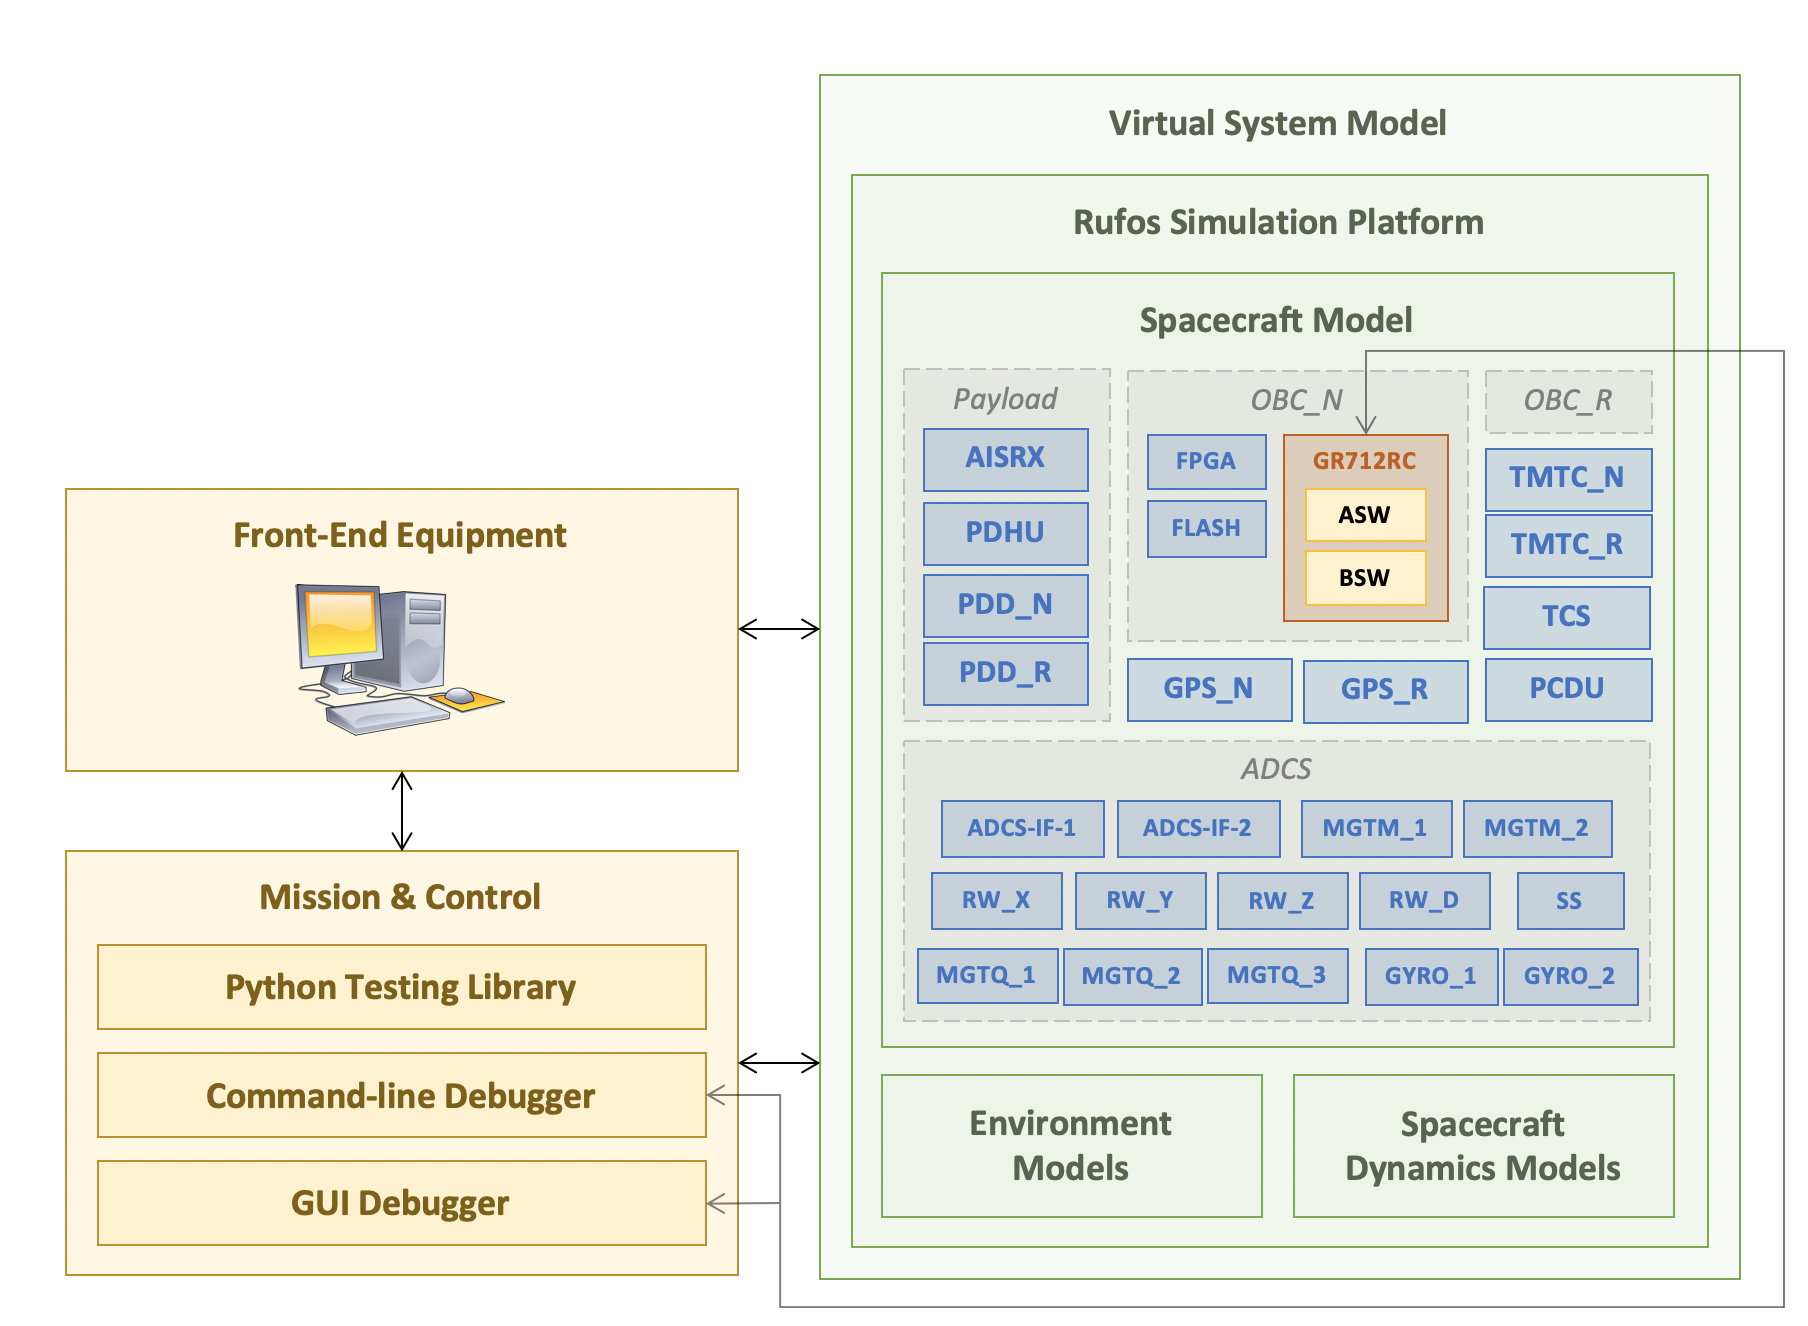
\includegraphics[width=0.7\textwidth]{images/esail}
    \caption{ESAIL system testing environment.}
    \label{fig:esail_case_study}
\end{figure}
 
The SVF simulator has been used for functional validation of the ESAIL CSW (see Figure~\ref{fig:esail_case_study}). The SVF is indeed one of the main testing tools used in satellite projects. The SVF simulator can be seen as a testing facility that presents also its own dedicated test suite to ensure the correctness of the SVF models and assembly to avoid later misunderstanding of the expected behaviours of the satellite CSW. 
In the context of the FAQAS project we consider the system test suite for the validation of the CSW, which are implemented using the SVF as the driving tool.
%Therefore, the SVF Simulator enables the evaluation of the FAQAS framework against two test suites: (1) the Test Suite of the SVF Simulator that validates the Simulator itself, (2) the system tests for the validation of CSW, which are implemented using the SVF as the driving tool.

Details about ESAIL are provided in the document \emph{FAQAS-LXS-MAN-001\_1- SVF Software Installation and User Manual} uploaded on Alfresco.

ESAIL is the largest case study system in FAQAS, the software consists of 924 source files with a total size of 187\,116 LOC. The system test suite consists of 121 python test scripts with a total of 384 sub-test cases. 
\MREVISION{C-P-22}{The system test suite takes up to 10 hours to finish its execution; the total execution time may be different and depends on the processing power of the computer where the SVF is being executed.}

\subsubsection{ESAIL System Test Suite Environment}

Because of the objectives of the project, we will need to execute a large number of mutants. Even if strategies for simplifying and reducing the number of mutants are designed (see Section~\ref{sec:approach}), there is a need for an infrastructure for running several mutant executions on parallel, which particularly applies for the ESAIL System Test Suite (e.g., the test suite execution time is high).

The University of Luxembourg provides a High-Performance Computing platform for academic purposes\footnote{https://hpc.uni.lu}.
The HPC has a computing capacity of 690 nodes, totaling 11\,280 computing cores, and a storage capacity of 8\,742 TB.

Given that ESAIL runs on a simulator (i.e., SVF), which is compute-intensive, and that resources of the UL HPC are shared between multiple jobs, non-deterministic behaviors are seldom observed (e.g., test cases fail because of lack of resources).

In view of the code-driven mutation testing process, where the quality of a test suite is assessed by checking if an injected fault is detected by the existing test cases, we need a test suite with a deterministic behavior, that is, if a test case fails it exclusively depends if we have introduced an artificial fault (i.e., a code mutation), and not because of the running environment.

To ensure that a mutant has been actually killed when executing the ESAIL System Suite on the UL HPC, we propose to execute a test case up to 10 times. If for any of this 10 executions the mutant is not killed, we consider it a live mutant. Otherwise, if it fails 10 times, we consider it a killed mutant.


Detailed information about the ESAIL system is provided in the following documents shared on Alfresco:

\begin{itemize}
	\item \emph{FAQAS-LXS-MAN-001\_1- SVF Software Installation and User Manual.pdf}, installation and testing instructions of the virtual machine containing ESAIL
	\item \emph{ESAIL-LXS-SDD-P-0105\_1B On-board Application Software Design Document.docx}, specifications document for the on-board system.
	\item \emph{ESAIL-LXS-ICD-P-0184\_2A ADCS IF SW External ICD.docx}, specifications document for the ADCS software.
	\item \emph{MOC-applicable MIB egos-mcs-s2k-icd-0001-version7.0-FINAL.pdf},  interface control document of the data import into SCOS-2000 run-time database, which is used to specify  the nominal value ranges for ESAIL ADCS parameters.
	\item \emph{ocp.dat}, text file for the SCOS-2000 Database Import ICD, containing the specifications of the nominal value ranges for ESAIL ADCS parameters.
\end{itemize}	


\subsection{Code-driven mutation testing}
\label{lxs:esail:system:codeDriven}

%\TODO{Code coverage information: we need Yago to produce a new code coverage report with VCAST.}

\REVNOV{PTCR-34}{The code-driven mutation testing process in ESAIL will be performed in two stages. First we will use a subset of ESAIL ($\mathit{ESAIL}_S$) to evaluate the accuracy of the estimated mutation score (see Section~\ref{sec:evaluation}). Then, in later stages, we will apply the approach (including mutants sampling, which is necessary for scalability purposes) to the whole ESAIL in order to (1) compare the mutation score obtained with the whole system with the mutation score obtained with $\mathit{ESAIL}_S$, (2) evaluate the accuracy of our strategy for removing equivalent/redundant mutants when applied to the whole ESAIL, (3) compare the mutation score obtained for the whole $ESAIL$ and for $\mathit{ESAIL}_S$ after removing likely equivalent and likely redundant mutants.}

\REVNOV{PTCR-34}{$\mathit{ESAIL}_S$ had been selected by LXS engineers by identifying representative source files that belong to the following categories: (1) source files that are used almost all the time by the test cases (i.e., files implementing service/protocol layer functions), (2) critical functions of the satellite implemented in high-level drivers, (3)  higher level application level functions.}

\STARTCHANGEDNOV
The files included in $\mathit{ESAIL}_S$ are:
\begin{itemize}
\item \emph{HighLevelDriverLayer/TMTC\_SYS\_Handler/Source/tmtchdl\_TmTcSysHandlerTask.c}
\item \emph{ProtocolLayer/TCFrameReader/Source/TCFrameReader.c}
\item \emph{ProtocolLayer/TMFrameBuilder/Source/TMFrameBuilder.c}
\item \emph{ServiceLayer/PUS\_1/Source/pus1\_GenerateReport.c}
\item \emph{ServiceLayer/PUS\_3/Source/pus3\_GenerateHkGroupReport.c}
\item \emph{ServiceLayer/PUS\_3/Source/pus3\_ExecuteTc\_3\_129.c}
\item \emph{ServiceLayer/PUS\_128/Source/pus128\_ExecuteTc\_128\_1.c}
\item \emph{ServiceLayer/PUS\_130/Source/pus130\_ExecuteTc\_130\_1.c}
\item \emph{ApplicationLayer/Operational\_Sequences/Source/SpacecraftConfigurationVector.c}
\item \emph{ApplicationLayer/Operational\_Sequences/Source/Transition\_To\_OPM.c}
\end{itemize}
\ENDCHANGEDNOV

Concerning the experiments conducted on the whole ESAIL, they will target all the components of the ESAIL on-board software, these components are:

\begin{itemize}
	\item ADCS
	\item CAN
	\item EPS
	\item FDIR
	\item OPSE
	\item SERVICES
	\item TCS
	\item TMTC
\end{itemize}

Code coverage information concerning the system-level test suite used for FAQAS is reported in \emph{FAQAS-LXS-MAN-001\_1- SVF Software Installation and User Manual.pdf}.


\subsection{Data-driven mutation testing}

A detailed description of the application of data-driven mutation testing to ESAIL is provided in APPENDIX~\ref{appendix:FMS}.

\section{LXS - ESAIL Unit Test Suite}
\label{chapter:caseStudies:LXS:Unit}



The unit test suite of ESAIL will be considered for the evaluation of the final FAQAS toolset. 
%For example, it is a possible case to be used for an independent use of the FAQAS framework by LXS engineers. The ESAIL unit test suite is used mainly to test critical functionalities of ESAIL components. The ESAIL unit test suite has been provided to ESA; however, the mutation testing activity might concern a subset of them. Indeed, evaluating with mutation testing a set of test cases that are known for covering only a subset of the features of the system might be of little usefulness. 
%%The set of test cases and functions to be tested will be provided along with the description of the achieved results at the end of WP3.
To assess the quality of the ESAIL unit test suite we will analyze the same ESAIL sub-system defined in Section~\ref{lxs:esail:system:codeDriven}, and thus, we will target the same set of mutants. Since the ESAIL Unit Test Suite has been implemented by LXS to cover scenarios hard to cover with a full simulation (consequently, it cover a limited portion of the code), we will use the ESAIL Unit Test Suite to provide a complementary analysis to the one given by the system test suite.



% !TEX root = MAIN.tex

\clearpage

\section{GSL - libgcsp}
\label{sec:caseStudies:GSL:libgcsp}

\subsection{Overview of the case study}

The GomSpace CSP library (libgscsp) is a GomSpace extension to the open source CubeSat Space Protocol library.
The GomSpace CSP library provides:
\begin{itemize}
\item convenience wrapping of CSP functionality, primarily initialization.
\item definition of standard CSP ports (used by other GomSpace products).
\item connecting low-level drivers (e.g. CAN, I2C from Embed library) with CSP interfaces 
\item generic CSP service dispatcher, forwards incoming connections to service handlers.
\end{itemize}

The libgscsp contains a GomSpace branch (https://github.com/GomSpace/libcsp) of the open source libcsp (https://github.com/libcsp/libcsp), located in the subfolder lib/libcsp. The two libcsp branches are kept as identical as possible, as features specific to GomSpace are placed in libgscsp.

Details about libgscsp are provided in the document \emph{gs-man-nanosoft-ms100-command-and-management-sdk-3.6.2-1-g67fe6e1.pdf} uploaded on Alfresco.


The size of libgscsp is 1\,497 LOC, %include 306, src 1776+15 = total = 1497
while libcsp (GSL branch) is 8\,339 LOC. % 6789 + 1550
Instead, the libgscsp unit test suite consists of 89 test cases, compiled and executed through the WAF meta-build system.

\subsection{Code-driven mutation testing}

\DONE{Can we provide separate information about the code coverage for libgscsp (no libcsp branch) and for libcsp branch?}

\DONE{Clarify which components we mutate}

We have seen that a mutant can be killed only if it is covered by at least one test case. For this reason, the code-driven mutation testing process in libgscsp will target all the components covered by the libgscsp unit test suite.

% !TEX root = ../MAIN.tex

\begin{table}[h]

\footnotesize
\parbox{.45\linewidth}{
\centering
\begin{tabular}{|l|l|}
\hline
\textbf{Coverage Type} & \textbf{Coverage Rate} \\
\hline
Statement     & 58.4\% (390 of 668 statements)\\
Functions     & 71.4\% (50 of 70 functions)\\
Branches      & 41.2\% (165 of 400 branches)\\
\hline
\end{tabular}
\caption{libgscsp code coverage.}
\label{table:libgscsp_coverage}
}
\hfill
\parbox{.45\linewidth}{
\centering
\begin{tabular}{|l|l|}
\hline
\textbf{Coverage Type} & \textbf{Coverage Rate} \\
\hline
Statement     & 64.1\% (2112 of 3297 statements)\\
Functions     & 72.5\% (248 of 342 functions)\\
Branches      & 44.9\% (989 of 2201 branches)\\
\hline
\end{tabular}
\caption{libcsp code coverage.}
\label{table:libcsp_coverage}
}
\end{table}	

\begin{enumerate}
	\item \textbf{libgscsp}

	Table~\ref{table:libgscsp_coverage} provides code coverage information of the libgscsp unit test suite for the GSL extension to the CSP library. Given the code coverage, we focus our analysis to the following subset of components (i.e., components with code coverage greater than 0\%):

	\begin{itemize}
	 	\item src/clock.c
	 	\item src/commands.c
	 	\item src/conn.c
	 	\item src/csp.c
	 	\item src/error.c
	 	\item src/log.c
	 	\item src/router.c
	 	\item src/service\_dispatcher.c
	 	\item src/service\_handler.c
	 	\item src/linux/command\_line.c

	 \end{itemize} 

	\item \textbf{libcsp (GSL branch)}

	Table~\ref{table:libcsp_coverage} presents the code coverage of the libgscsp unit test suite for the GSL branch of the CSP library.  Given the code coverage, we focus our mutation analysis on the following subset of components (i.e., components with code coverage greater than 0\%):

	\begin{itemize}
		\item src/arch/csp\_time.c
		\item src/arch/csp\_system.c
		\item src/arch/posix/csp\_thread.c
		\item src/arch/posix/csp\_semaphore.c
		\item src/arch/posix/csp\_malloc.c
		\item src/arch/posix/csp\_queue.c
		\item src/arch/posix/csp\_time.c
		\item src/arch/posix/pthread\_queue.c
		\item src/arch/posix/csp\_system.c
		\item src/crypto/csp\_sha1.c
		\item src/crypto/csp\_hmac.c
		\item src/crypto/csp\_xtea.c
		\item src/interfaces/csp\_if\_lo.c
		\item src/rtable/csp\_rtable.c
		\item src/rtable/csp\_rtable\_cidr.c
		\item src/rtable/csp\_rtable\_static.c
		\item src/transport/csp\_rdp.c
		\item src/transport/csp\_udp.c
		\item src/csp\_sfp.c
		\item src/csp\_debug.c
		\item src/csp\_service\_handler.c
		\item src/csp\_crc32.c
		\item src/csp\_io.c
		\item src/csp\_qfifo.c
		\item src/csp\_iflist.c
		\item src/csp\_endian.c
		\item src/csp\_route.c
		\item src/csp\_buffer.c
		\item src/csp\_port.c
		\item src/csp\_conn.c
		\item src/csp\_init.c
		\item src/csp\_services.c
	\end{itemize}


\end{enumerate}

\subsubsection{Mutation Testing Preliminary Results}

\DONE{We can add some preliminary results}

% !TEX root = ../MAIN.tex

\begin{table}[h]
\small
\centering
\caption{Code-driven mutation testing preliminary results for the libgscsp case study.}
\label{table:libgscsp_preliminary}
\begin{tabular}{|l|l|l|l|l|l|l|}
\hline
        & \multicolumn{5}{c|}{Mutants}                                                                      & \multirow{3}{*}{\begin{tabular}[c]{@{}l@{}}Mutation Score\\ (K/K+L)\end{tabular}} \\ \cline{1-6}
        &     &                                                        &      & \multicolumn{2}{c|}{Killed} &                                                                                   \\ \cline{1-6}
Mutants & All & \begin{tabular}[c]{@{}l@{}}Not\\ Compiled\end{tabular} & Live & Test Failure    & Timeout   &                                                                                   \\ \hline
Total   &  6\,196   &  1\,700 & 1\,708      & 2\,495                & 277          & 61.88\%                                                                           \\ \hline
\end{tabular}
\end{table}    
             

In order to analyze the feasibility of the code-driven mutation testing for libgscsp, we conducted a preliminary experimentation using the mutation operators AOR, ROR, ICR, LCR, ABS, UOI and SDL we generated 6\,196 mutants. For the experimentation we consider only the libcsp (GSL branch) source code. Preliminary results can be found in Table~\ref{table:libgscsp_preliminary}.
Particularly, we observe that from the 6\,196 generated mutants, we had 1\,700 mutants that were not compiled by the compilation toolset of libgscsp, most probably because the mutation introduced a syntactical error that was detected by the toolset.
Then, we identified 1\,708 live mutants that were not detected by the test suite. Instead, we had 2\,495 killed mutants detected by the test suite, and 277 mutants that produced libutil to go into an infinite loop, and thus were killed by timeout. The final mutation score was of 61.88\%.

The identification of equivalent mutants still needs to be assessed.


\subsection{Data-driven mutation testing}

\DONE{We should indicate the functions we mutate.}

The data-driven mutation testing process in libgscsp will target the data packet transferred between the server and the client using the CSP protocol. Specifically, the mutations will affect the header of the packet, in general the routing information (see Figure~\ref{fig:csp_packet}), and the payload of the packet.

\begin{figure}[h]
  \centering
    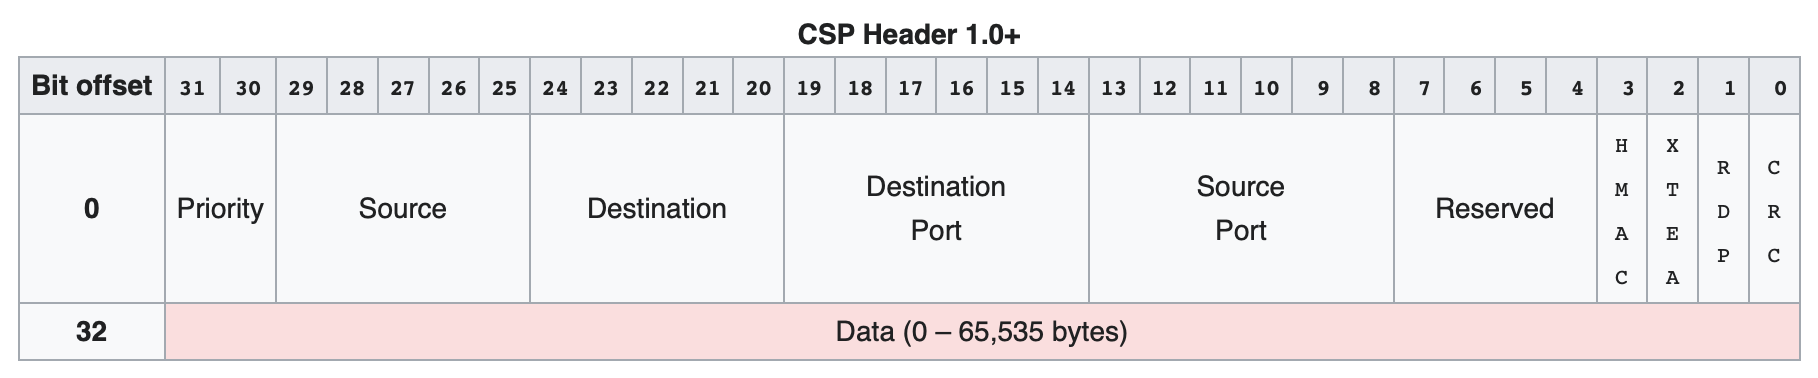
\includegraphics[width=0.9\textwidth]{images/csp_packet}
      \caption{CSP protocol header.}
      \label{fig:csp_packet}
\end{figure}


% !TEX root =  ../MAIN.tex

\begin{minipage}{16cm}
\begin{lstlisting}[style=CStyle, caption=Data-driven mutation example on libgscsp (csp\_io.c excerpt)., label=csp_integration]
unsigned int v[6] = {packet->id.flags, packet->id.sport, packet->id.dport, 
                    packet->id.dst, packet->id.src, packet->id.pri};

FaultModel *fm = _FAQAS_Identifier_FM();                                                                                          
mutate(v, fm);
_FAQAS_delete_FM(fm);

packet->id.flags = v[0];
packet->id.sport = v[1];
packet->id.dport = v[2]; 
packet->id.dst = v[3]; 
packet->id.src = v[4]; 
packet->id.pri = v[5]; 
\end{lstlisting}
\end{minipage}


Both mutations (i.e, header and payload) will be performed before the message is serialized. 
For example, the mutations to the header will affect the csp\_send\_direct function of the csp\_io component. Listing~\ref{csp_integration} shows an example of our data-driven mutator prototype within the csp\_io component. Particularly, the packet header is translated into an unsigned int vector, which is then passed to the FAQAS mutate function, here a fault model could be applied to all six items of the header. After the mutation is applied the vector is translated back again to the original representation.
 

\section{GSL - libparam}
\label{sec:caseStudies:GSL:libparam}

\subsection{Overview of the case study}

The Parameter System (i.e., libparam) is a light-weight parameter system designed for GomSpace satellite subsystems. It is based around a logical memory architecture, where every parameter is referenced directly by its logical address. A backend system takes care of translating addresses into physical addresses.
The features of this system include:
\begin{itemize}
\item Direct memory access for quick parameter reads.
\item Simple data types: uint, int, float, double, string.
\item Arrays of simple data types.
\item Supports multiple stores per table, e.g. FRAM, MCU flash, file (binary or text).
\item Remote client with support for most features (rparam).
\item Packed GET, SET queries, supporting multiple parameter set/get in a single request. Data serialization and deserialization.
\item Supports both little and big-endian systems.
\item Commands for both local (param) and remote access (rparam).
\item Parameter server for remote access over CSP.
\item Compile-time configuration of parameter system
\end{itemize}

Details about libparam are provided in the document \emph{gs-man-nanosoft-ms100-command-and-management-sdk-3.6.2-1-g67fe6e1.pdf} uploaded on Alfresco.

\subsection{Code-driven mutation testing}

\TODO{We do it or not?}

\subsection{Data-driven mutation testing}

\TODO{We should indicate the functions we mutate}


\section{GSL - libutil}
\label{sec:caseStudies:GSL:libutil}

\subsection{Overview of the case study}

The Utility library provides cross-platform APIs for common functionality, for use in both embedded systems and standard PCs running Linux. 

Details about libutil are provided in the document \emph{gs-man-nanosoft-ms100-command-and-management-sdk-3.6.2-1-g67fe6e1.pdf} uploaded on Alfresco.

The size of libutil is 10\,576 LOC, while the unit test suite consists of 201 test cases written in C.

\subsection{Code-driven mutation testing}

\DONE{Add some details about what we mutated}

The code-driven mutation testing process in libutil will target all the components covered by the libutil unit test suite. 

% !TEX root = ../MAIN.tex

\begin{table}[h]

\centering
\begin{tabular}{|l|l|}
\hline
\textbf{Coverage Type} & \textbf{Coverage Rate} \\
\hline
Statement     & 83.2\% (8\,817 of 10\,596 statements)\\
Functions     & 82.1\% (725 of 883 functions)\\
Branches      & 56.6\% (2\,618 of 4\,627 branches)\\
\hline
\end{tabular}
\caption{libutil code coverage.}
\label{table:gslibutil_coverage}

\end{table}

Table~\ref{table:gslibutil_coverage} provides the code coverage information of the unit test suite for the GSL libutil library. Given the code coverage, we focus our analysis to the following subset of components (i.e., components with code coverage greater than 0\%):

\begin{itemize}
	\item src/base16.c
	\item src/bytebuffer.c
	\item src/byteorder.c
	\item src/clock.c
	\item src/crc32.c
	\item src/crc8.c
	\item src/error.c
	\item src/fletcher.c
	\item src/function\_scheduler.c
	\item src/hexdump.c
	\item src/lock.c
	\item src/rtc.c
	\item src/string.c
	\item src/strtoint.c
	\item src/time.c
	\item src/timestamp.c
	\item src/cmd/command.c
	\item src/cmd/log.c
	\item src/cmd/vmem.c
	\item src/drivers/sys/memory.c
	\item src/gosh/command.c
	\item src/gosh/console.c
	\item src/gosh/default\_commands.c
	\item src/linux/clock.c
	\item src/linux/command\_line.c
	\item src/linux/cwd.c
	\item src/linux/delay.c
	\item src/linux/function.c
	\item src/linux/mutex.c
	\item src/linux/queue.c
	\item src/linux/rtc.c
	\item src/linux/sem.c
	\item src/linux/signal.c
	\item src/linux/stdio.c
	\item src/linux/thread.c
	\item src/linux/time.c
	\item src/linux/drivers/gpio/gpio.c
	\item src/linux/drivers/gpio/gpio\_sysfs.c
	\item src/linux/drivers/gpio/gpio\_virtual.c
	\item src/linux/drivers/i2c/i2c.c
	\item src/linux/drivers/spi/spi.c
	\item src/linux/drivers/sys/memory.c
	\item src/log/commands.c
	\item src/log/log.c
	\item src/log/appender/console.c
	\item src/log/appender/simple\_file.c
	\item src/test/cmocka.c
	\item src/test/command.c
	\item src/test/log.c
	\item src/vmem/commands.c
	\item src/vmem/vmem.c
	\item src/watchdog/monitor\_task.c
	\item src/watchdog/watchdog.c
	\item src/zip/zip.c
	\item src/zip/miniz/miniz.c
\end{itemize}

\subsubsection{Mutation Testing Preliminary Results}

\DONE{We can add some preliminary results}

% !TEX root = ../MAIN.tex

\begin{table}[h]
\small
\centering
\caption{Code-driven mutation testing preliminary results for the libutil case study.}
\label{table:libutil_preliminary}
\begin{tabular}{|l|l|l|l|l|l|l|}
\hline
        & \multicolumn{5}{c|}{Mutants}                                                                      & \multirow{3}{*}{\begin{tabular}[c]{@{}l@{}}Mutation Score\\ (K/K+L)\end{tabular}} \\ \cline{1-6}
        &     &                                                        &      & \multicolumn{2}{c|}{Killed} &                                                                                   \\ \cline{1-6}
Mutants & All & \begin{tabular}[c]{@{}l@{}}Not\\ Compiled\end{tabular} & Live & Test Failure    & Timeout   &                                                                                   \\ \hline
Total   &  16\,886   &  2\,561                                                      & 3\,402      & 10\,634                & 289          & 76.25\%                                                                           \\ \hline
\end{tabular}
\end{table}    
             

In order to analyze the feasibility of the code-driven mutation testing, we conducted a preliminary experimentation using the mutation operators AOR, ROR, ICR, LCR, and SDL we generated 16\,886 mutants. Preliminary results can be found in Table~\ref{table:libutil_preliminary}.
Particularly, we observe that from the 16\,886 generated mutants, we had 2\,561 mutants that were not compiled by the compilation toolset of libutil, most probably because the mutation introduced a syntactical error that was detected by the toolset.
Then, we identified 3\,402 live mutants that were not detected by the test suite. Instead, we had 10\,634 killed mutants detected by the test suite, and 289 mutants that produced libutil to go into an infinite loop, and thus were killed by timeout. The final mutation score was of 76.25\%.

The identification of equivalent mutants still needs to be assessed.


\subsection{Data-driven mutation testing}

We do not plan to apply data drive mutation testing to this case study because is a standalone library; it does not integrate communicating components.



% !TEX root = MAIN.tex
\clearpage

\section{MLFS}
\label{sec:caseStudies:GSL:MLSF}

\subsection{Overview of the case study}

The \INDEX{Mathematical Library for Flight Software} (MLFS) implements mathematical functions ready for qualification. 
%\DONE{Please rewrite the following sentence}
MLFS is born from the need of having a mathematical library ready for qualification for flight software. Well known mathematical libraries such as \texttt{libm}~\cite{libm} and \texttt{newlib}~\cite{newlib} are not completely validated with respect to specific input ranges, errors and performance, and so, they do not comply with ECSS criticality category B.
The set of functions provided by MLFS are limited to the functions typically needed in flight software. 


The source code size is 5\,402 LOC, while the unit test suite consists of 4\,042 tests for 92 functions.



% !TEX root = MAIN.tex

\clearpage

\section{ASN1SCC}
\label{sec:caseStudies:GSL:ASN1}

\subsection{Overview of the case study}

ASN1SCC is an open source ASN.1 compiler that generates C/C++ and SPARK/Ada code suitable for low resource environments such as space systems. Moreover, the compiler can produce a test harness that provides full statement coverage in the generated code, and therefore significantly improves its quality.

Details about ASN.1 compiler are provided in the document \emph{taste-documentation-current.pdf} uploaded on Alfresco.

In the context of FAQAS, we focus our analysis on the auto-generated source code by the ASN.1 compiler, rather than in ASN1SCC software itself.

For the definition of the ASN.1 compiler case study, we introduce the example of a specific grammar. An excerpt of such grammar is shown in Listing~\ref{asn_excerpt}. 
The excerpt of the grammar introduces the definition of six data types, each data type also specifies the expected constraint, for example, the data type \texttt{MyInt} is an INTEGER which can have values from 0 to 20. The full source code of the grammar can be found in the file \emph{test.asn} uploaded on Alfresco.

For the given grammar, the size of the auto-generated source code is 4\,338 LOC. While the unit test suite consists of 107 auto-generated test cases.

% !TEX root =  ../MAIN.tex

\begin{minipage}{15cm}
\begin{lstlisting}[style=CStyle, caption=Excerpt of the tested ASN1 grammar., label=asn_excerpt, mathescape=true]
MyInt ::= INTEGER (0 .. 20)

My2ndInt ::= MyInt ( 1 .. 18)

AType ::= SEQUENCE {
    blArray SEQUENCE (SIZE(10)) OF BOOLEAN
}

My2ndAType ::= AType

TypeNested ::= SEQUENCE {
    intVal  INTEGER(0..10),
    int2Val INTEGER(-10..10),
    int3Val MyInt (10..12),
    intArray    SEQUENCE (SIZE (10)) OF INTEGER (0..3),
    realArray   SEQUENCE (SIZE (10)) OF REAL (0.1 .. 3.14),
    octStrArray SEQUENCE (SIZE (10)) OF OCTET STRING (SIZE(1..10)),
    boolArray   SEQUENCE (SIZE (10)) OF T-BOOL,
    label   OCTET STRING (SIZE(10..40)),
    bAlpha  T-BOOL,
    bBeta   BOOLEAN,
    sString T-STRING,
    arr     T-ARR,
    arr2    T-ARR2
}

E ::= INTEGER (0..255|1299)(5)
\end{lstlisting}
\end{minipage}



\subsection{Code-driven mutation testing}

% !TEX root = ../MAIN.tex

\begin{table}[h]

\centering
\begin{tabular}{|l|l|}
\hline
\textbf{Coverage Type} & \textbf{Coverage Rate} \\
\hline
Statement     & 83.7\% (2\,718 of 3\,246 statements)\\
Functions     & 87.4\% (285 of 326 functions)\\
Branches      & 51.2\% (1\,233 of 2\,407 branches)\\
\hline
\end{tabular}
\caption{ASN.1 grammar code coverage.}
\label{table:asn1grammar_coverage}

\end{table}



The objective of this case study is to provide ASN1SCC engineers tangible evidence on how to improve the auto-generated test cases, by reporting detailed information of live mutants and possible candidates of new test cases. In this manner, the quality of test suites of embedded systems that includes the auto-generated source code from ASN.1, can also be improved.

Table~\ref{table:asn1grammar_coverage} provides the code coverage information of the auto-generated source code of the \emph{test.asn} grammar. Given the code coverage, we focus our code-driven mutation testing analysis to the following subset of components (i.e., components with code coverage greater than 0\%):

\begin{itemize}
	\item asn1crt\_encoding.c: implementation of the ASN.1 constraints encoding/decoding procedures.
	\item test.c: implementation of the grammar data types encoding/decoding procedures.
	\item test\_auto\_tcs.c: wrapper of the grammar data types encoding/decoding procedures used in the test cases.
\end{itemize}

\subsubsection{Mutation Testing Preliminary Results}

% !TEX root = ../MAIN.tex

\begin{table}[h]
\small
\centering
\caption{Code-driven mutation testing preliminary results for the ASN.1 case study.}
\label{table:asn1_preliminary}
\begin{tabular}{|l|l|l|l|l|l|l|}
\hline
        & \multicolumn{5}{c|}{Mutants}                                                                      & \multirow{3}{*}{\begin{tabular}[c]{@{}l@{}}Mutation Score\\ (K/K+L)\end{tabular}} \\ \cline{1-6}
        &     &                                                        &      & \multicolumn{2}{c|}{Killed} &                                                                                   \\ \cline{1-6}
Mutants & All & \begin{tabular}[c]{@{}l@{}}Not\\ Compiled\end{tabular} & Live & Test Failure    & Timeout   &                                                                                   \\ \hline
Total   &  9\,174   &  1\,215   & 4\,263      & 3\,009                & 687          & 53.56\%                                                                           \\ \hline
\end{tabular}
\end{table}    
             

In order to analyze the feasibility of the code-driven mutation testing for ASN.1, we conducted a preliminary experimentation using the mutation operators AOR, ROR, ICR, LCR, ABS, UOI and SDL we generated 9\,174 mutants. Preliminary results can be found in Table~\ref{table:asn1_preliminary}.
Particularly, we observe that from the 9\,174 generated mutants, we had 1\,215 mutants that were not compiled by the compilation toolset of ASN.1, most probably because the mutation introduced a syntactical error that was detected by the toolset.
Then, we identified 4\,263 live mutants that were not detected by the test suite. Instead, we had 3\,009 killed mutants detected by the test suite, and 687 mutants that produced libutil to go into an infinite loop, and thus were killed by timeout. The final mutation score was of 53.56\%.

The identification of equivalent mutants still needs to be performed.


\subsection{Data-driven mutation testing}

In the context of this project, we foresee two scenarios on how to apply the data-driven mutation testing approach to the ASN.1 case study system. 

\subsubsection{Scenario 1: Testing the ASN.1 Compiler}

The first scenario simply automates robustness testing for ASN.1; we aim to rely on the automatically generated configuration parameters for mutation operators to generate data values that do not respect such constraints. This enables to verify the capability of the ASN.1 code to verifies the constraints of the data types defined in ASN.1 grammars.





%In the first scenario, we focus on the robustness of the auto-generated test cases of an ASN.1 grammar through the ASN.1 compiler.
%Particularly, we aim to apply a fault model that enables different mutations on the data types automatically generated by the ASN.1 compiler. Consequently, for every data type defined in the ASN.1 grammar, we automatically generate a set of probes that stresses all the data types constraints, where each probe contains a single instance of the defined fault model.
%
%The full description of the fault model can be found in Section~\ref{subsub:asn1model}.

\subsubsection{Scenario 2: Testing Case Study Systems using ASN.1}

%The second scenario aims to stress test suites from software systems that uses the encoding and decoding procedures derived from the ASN.1 compiler.
%
%More details about each scenario is provided in the following.

In this second scenario, we aim to assess the adequacy of test suites from software systems that embed the decoding and decoding auto-generated source code from ASN.1 grammar through the ASN.1 compiler.

For this task, we will ask engineers to specify fault models to decide what mutation operator to apply for each data type defined in the ASN.1 grammar.
Additionally, the engineer will be asked to specify in the fault model the nominal ranges for each data type; after applying a specific mutation operator, we will assess if the existing test suite is able to detect the corresponding mutated value by killing the introduced mutant.

For this scenario, further discussions with ESA are required in order to identify case study systems using the ASN.1 compiler. 




